\documentclass[a4paper,11pt,landscape,twocolumn]{article}

\usepackage{préambule}
\usepackage{clipboard}
\usetikzlibrary{arrows.meta}

\makeatletter
\renewcommand{\maketitle}{%
{\scriptsize colle dans ton cahier d'exercices}
	\begin{center}
		\LARGE
		\uline{\@title}
		\vspace{0.5em}
	\end{center}
}
\makeatother

\title{Bonus : d'autres nombres}
\date{}
\author{}

\begin{document}

\Copy{nombres}{
	On va essayer de placer des nombres plus étranges sur la droite graduée suivante : \vspace{2em}

	\begin{center}
		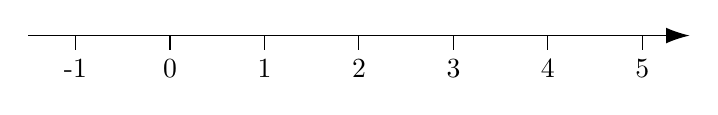
\begin{tikzpicture}[scale=1.2]
			\draw[-{Latex[length=3mm, width=2mm]}] (-1.5,0) -- (5.5,0);
			\foreach \x in {-1,...,5} {
					\draw (\x,0) -- (\x,-0.15) node[below] {\x};
				}
		\end{tikzpicture}
	\end{center}

	\begin{enumerate}
		\item Reproduit cette droite graduée dans ton cahier.
		\item Dans la figure suivante, le côté [BC] a pour longueur \\ $\sqrt{2} = 1{,}414213⋯$

		      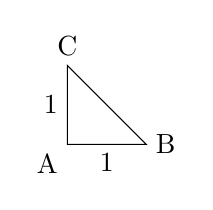
\begin{tikzpicture}
			      \draw (0,0) node[below left] {A}
			      -- node[below] {1} (1,0) node[right] {B}
			      -- (0,1) node[above] {C}
			      -- node[left] {1} cycle;
		      \end{tikzpicture}

		      Quel outil peux-tu utiliser pour placer le point R d'abscisse $\sqrt{2}$ sur la droite graduée ?
		\item On veut placer exactement le point F d'abscisse $\frac{1}{3}$.

		      \begin{itemize}
			      \item     Au dessus de la droite graduée, dessine un segment \textbf{parallèle à la droite graduée} de longueur 3 centimètres. Note A₁ son point d'extrêmité gauche, A₂ le point à 1 centimètre de la gauche, et A₃ son point d'extrêmité droite.
			      \item Trace une droite passant par A₁ et le point d'abscisse 0, et une droite passant par A₃ et le point d'abscisse 1.

			            Note I leur point d'intersection.
			      \item Trace la droite (A₂I). L'endroit où elle intersecte la droite graduée est le point d'abscisse $\frac{1}{3}$.
		      \end{itemize}
		\item (Question ouverte) Penses-tu qu'il est possible de placer exactement le point P d'abscisse π$=3{,}141592⋯$ ? Si oui, comment ferais-tu ?
	\end{enumerate}
}

\newpage

\Paste{nombres}

\end{document}